The relaxation of Section~\ref{sec:relax} has two ingredients that can each tighten the geography-free bound: connectivity of the cell support in the quotient graph, and the subdivision budget. To separate them we ran, for every (state, party, $q$), (a) the geography-free hull bound (one cell, no connectivity: the sorting bound of \citealt{duchin2019}, extended to $k$-way allocations and the whole spectrum), (b) the aggregated relaxation with counties as cells and connectivity but \emph{no budget}, (c) the same after two uniform levels of refinement (roughly four to ten times as many cells), and compared them with the certified bracket under the budget $s=k-1$ (Figure~\ref{fig:ablation}, Table~\ref{tab:ablation} in the appendix; for $k\ge3$ the relaxations (a)--(c) are the pool relaxations with one aggregate for the unsafe districts, which are also valid).

\begin{figure}[!tbp]
\centering
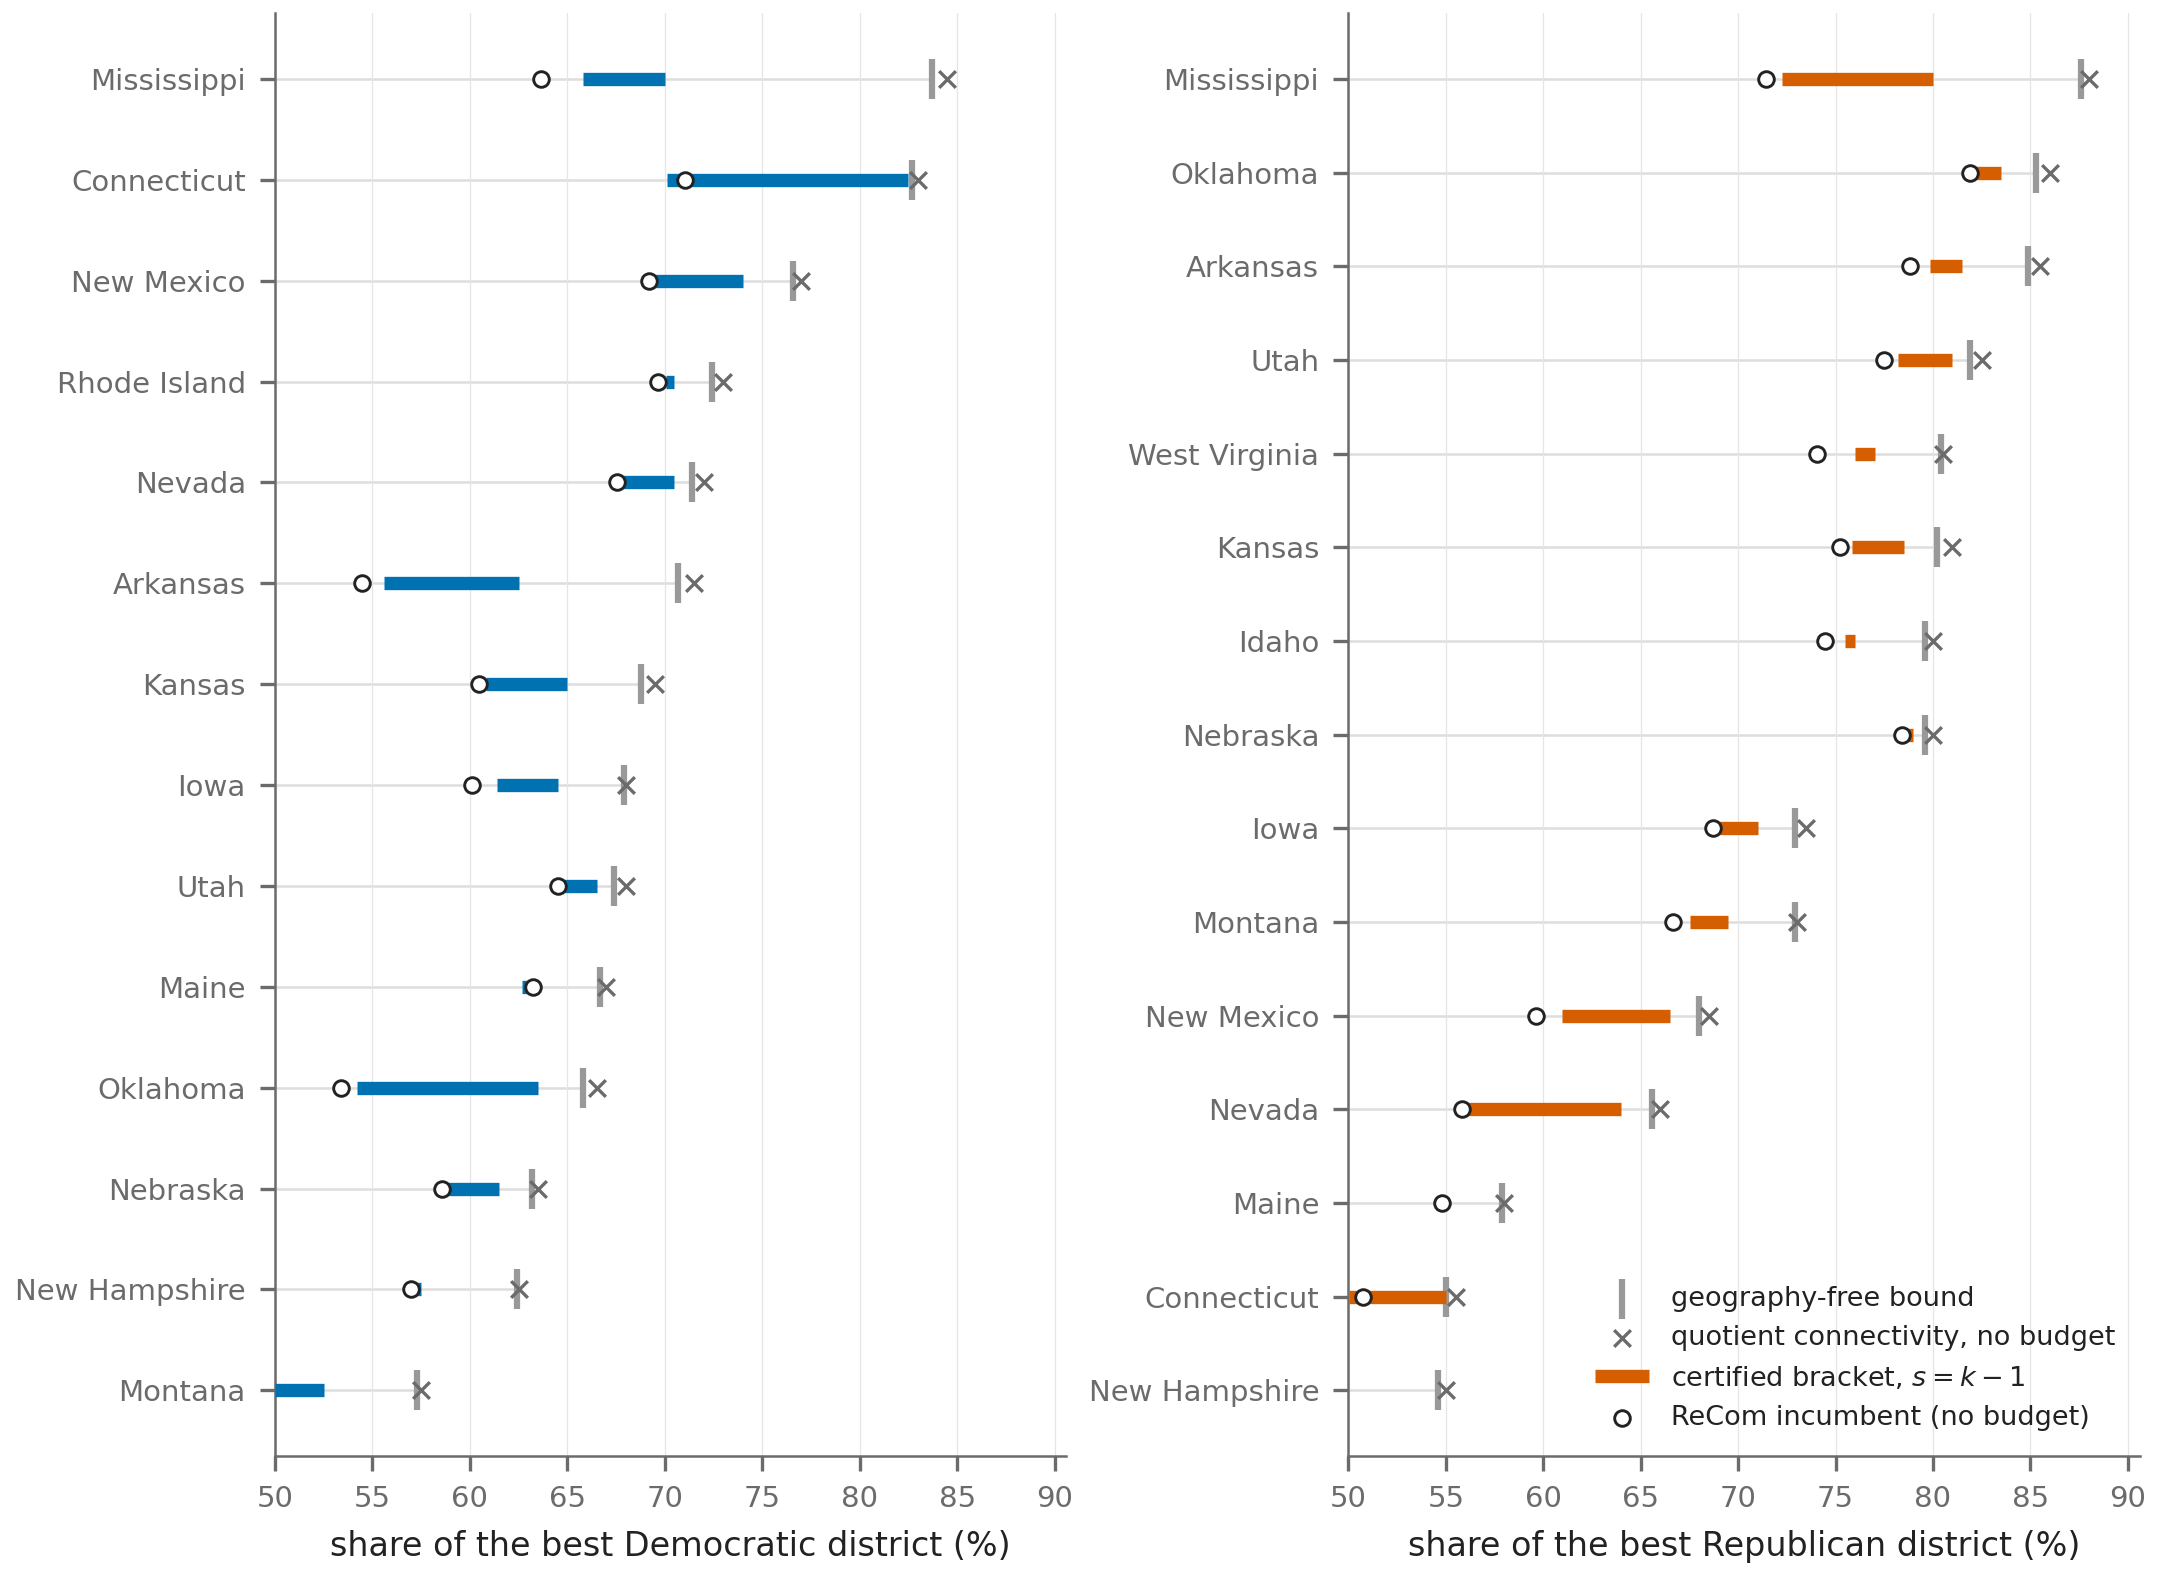
\includegraphics[width=\linewidth,height=0.68\textheight,keepaspectratio]{figs/ablation.png}
\caption{Upper bounds and incumbents for the share of the most extreme district ($q=1$), states with a nontrivial bound. Grey bar: geography-free hull bound; cross: quotient-connectivity relaxation with counties as cells and no budget (identical to within grid resolution after two further refinement levels); circle: 40-second unconstrained ReCom hill-climbing incumbent; thick bar: certified bracket under the budget of $k-1$ county splits.}\label{fig:ablation}
\end{figure}

\paragraph{Connectivity coarsening alone does nothing.}
Over the 79 nontrivial (state, party, $q$) triples the quotient relaxation without budget is never tighter than the geography-free bound (difference $+0.3$ point at the median, range 0.0 to $+0.8$, i.e. grid noise), and neither is it after two levels of refinement. This is the phenomenon of Proposition~\ref{prop:blind}: a district can touch every cell of a connected cell set while taking, in each cell, exactly its best atoms.

\paragraph{The budget does.}
The certified upper end under the budget is tighter than the geography-free bound by more than 0.05 point in 55 of the 78 triples with a finite upper end (median improvement 0.65 point; for $q=1$ the median is 2.75 points with a range from 0.2 to 13.7 points). Where it is not, the bracket is one of the open ones (Section~\ref{sec:main}) and the geography-free bound is used as the upper end (Table~\ref{tab:spectrum}). For the two-district states the improvement is decisive: New Hampshire Democrats 62.4\% $\to$ 57.0--57.5\%, Idaho Republicans 79.6\% $\to$ 75.5--76.0\%, West Virginia Republicans 80.4\% $\to$ 76.0--77.0\%.

\paragraph{Counting by pieces.}
Counting split \emph{counties} instead of pieces (a county cut among all districts costs one split) leaves a whole county as an unconstrained sub-problem. In development this was visible in Nebraska, where Douglas County holds 30\% of the state's population: under that convention the relaxed solutions of a query near the transition cut Douglas three ways for a single split, so that the exact problem contained a free three-way partition of 237 precincts, and CP-SAT alone could not even produce a feasible plan for $q=0$ within 300~s (a county-aware recombination heuristic finds one in milliseconds). We therefore adopted the piece-based count, which is also the convention of the exact county-split literature, and report only its results; we did not attempt a controlled comparison of the two conventions.
